\documentclass[10pt,journal,compsoc]{IEEEtran}

\ifCLASSINFOpdf
  \usepackage[pdftex]{graphicx}
  \graphicspath{{../pdf/}{../jpeg/}{../png/}}
  \DeclareGraphicsExtensions{.pdf,.jpeg,.png}
\else
  \usepackage[dvips]{graphicx}
  \graphicspath{{../eps/}}
  \DeclareGraphicsExtensions{.eps}
\fi

\usepackage{color}
\usepackage{mathtools}	% for \mathclap
\usepackage{amssymb}	%for mathbb{}
\usepackage{amsmath}
% Note that the amsmath package sets \interdisplaylinepenalty to 10000
% thus preventing page breaks from occurring within multiline equations. Use:
\interdisplaylinepenalty=2500

% *** ALIGNMENT PACKAGES ***
%
%\usepackage{array}
% Frank Mittelbach's and David Carlisle's array.sty patches and improves
% the standard LaTeX2e array and tabular environments to provide better
% appearance and additional user controls. As the default LaTeX2e table
% generation code is lacking to the point of almost being broken with
% respect to the quality of the end results, all users are strongly
% advised to use an enhanced (at the very least that provided by array.sty)
% set of table tools. array.sty is already installed on most systems. The
% latest version and documentation can be obtained at:
% http://www.ctan.org/pkg/array


%\usepackage{mdwmath}
%\usepackage{mdwtab}
% Also highly recommended is Mark Wooding's extremely powerful MDW tools,
% especially mdwmath.sty and mdwtab.sty which are used to format equations
% and tables, respectively. The MDWtools set is already installed on most
% LaTeX systems. The lastest version and documentation is available at:
% http://www.ctan.org/pkg/mdwtools


% IEEEtran contains the IEEEeqnarray family of commands that can be used to
% generate multiline equations as well as matrices, tables, etc., of high
% quality.


%\usepackage{eqparbox}
% Also of notable interest is Scott Pakin's eqparbox package for creating
% (automatically sized) equal width boxes - aka "natural width parboxes".
% Available at:
% http://www.ctan.org/pkg/eqparbox




% *** SUBFIGURE PACKAGES ***
%\ifCLASSOPTIONcompsoc
%  \usepackage[caption=false,font=footnotesize,labelfont=sf,textfont=sf]{subfig}
%\else
%  \usepackage[caption=false,font=footnotesize]{subfig}
%\fi
% subfig.sty, written by Steven Douglas Cochran, is the modern replacement
% for subfigure.sty, the latter of which is no longer maintained and is
% incompatible with some LaTeX packages including fixltx2e. However,
% subfig.sty requires and automatically loads Axel Sommerfeldt's caption.sty
% which will override IEEEtran.cls' handling of captions and this will result
% in non-IEEE style figure/table captions. To prevent this problem, be sure
% and invoke subfig.sty's "caption=false" package option (available since
% subfig.sty version 1.3, 2005/06/28) as this is will preserve IEEEtran.cls
% handling of captions.
% Note that the Computer Society format requires a sans serif font rather
% than the serif font used in traditional IEEE formatting and thus the need
% to invoke different subfig.sty package options depending on whether
% compsoc mode has been enabled.
%
% The latest version and documentation of subfig.sty can be obtained at:
% http://www.ctan.org/pkg/subfig



% *** PDF, URL AND HYPERLINK PACKAGES ***
\usepackage{url}
% url.sty was written by Donald Arseneau. It provides better support for
% handling and breaking URLs. url.sty is already installed on most LaTeX
% systems. The latest version and documentation can be obtained at:
% http://www.ctan.org/pkg/url
% Basically, \url{my_url_here}.

\newtheorem{thm}{Theorem}		% for theorem environment
\newtheorem{lem}[thm]{Lemma}		% for Lemma environment
\newtheorem{defn}[thm]{Definition}		% for Definition environment

\begin{document}

\title{A Comparison of Synchronous and Asynchronous Digital Design}

\author{Sohum Datta, EECS, UC Berkeley
\\sohumdatat@berkeley.edu 
\thanks{
This is the final report for the term project of EE241B: Advanced Digital Integrated
Circuits offered in Spring 2017 by Prof. Borivoje Nikolic at UC Berkeley,
CA 94704, United States. Special thanks to Vignesh Iyer and Prof. Elad Alon,
GSI and Instructor of EECS151/251 Spring 2017. The experiments would not have
been possible without their equipment and support.}}

\IEEEtitleabstractindextext{%

\begin{abstract}
A simple experiment is described which compares synchronous and
asynchronous implementations of a three-stage integer pipeline.
The aim of the experiment was to replicate some results of similar previous
works and gain insights to the fundamental difference between the two
paradigms. The asynchronous implementation was about 19\% worse in area
and 64\% worse in throughput than the synchronous design.
A derivation of the Muller C gate based on latches and a
proof of linearity of the lower bound on energy scalability with the
entropy of specification of asynchronous circuits is also provided.

This document is self-contained for the experimental setup. A summary of
design methods for asynchronous processors is also provided.
However, the proofs in appendices are brief and important results used are only
stated without derivations.

\end{abstract}



% Note that keywords are not normally used for peerreview papers.
\begin{IEEEkeywords}
 Asynchronous Circuits, Field-Programmable Gate Arrays, Self-timed Pipelines,
 Quasi-Delay Insensitive Circuits, prefix codes, process algebra.
\end{IEEEkeywords}}
\maketitle


\section{Introduction}

Asynchronous circuits have no clock. The sequencing of dependent computations
is done via \emph{handshaking}. 

The main advantage of asynchronous circuits is the inherent
\emph{slack-free} nature. The worst-case correctness behaviour for synchronous
systems is replaced by \emph{average}-case behaviour in asynchronous systems.

Synchronous circuits consume energy strongly related to the \emph{largest combinational
delay} in its path. By contrast, 
asynchronous circuits of large systems can be made to consume energy within a 
constant factor of the circuits entropy. A proof is outlined in Appendix B.

However, there are some serious pitfalls of this new paradigm.
For asynchronous circuits, Computer Aided Design (CAD) infrastructure is still in its infancy.
Estimating the average-case delay of a circuit 
is an NP-Hard problem \cite{seger_book}. It can also depend
on component delays in unexpected ways -- a faster gate can lead to overall
slower circuit! (For an example, please refer \cite{seger_book},
pg. 7). Finally, verification of asynchronous circuit can be very difficult 
\cite{async_test_survey}. A substantial family of circuit
classes cannot be tested for certain types of errors \cite{async_c_test}.

\section{Asynchronous Circuits on FPGA}

Prototyping asynchronous circuits on Field-Programmable Gate Arrays (FPGAs)
is a recent trend. As designers turn to explore asynchronous
circuits, the cheaper platform which is widely deployed in today's data-centers
serves better \cite{japan_fpga_paper}. Moreover, many modern systems features
(such as  Multi-Processor SoC, ARM IP Cores) can be easily
integrated with the  asynchronous circuit implemented.

There are several ways to design asynchronous circuits on commercial FPGAs 
\cite{japan_1} \cite{japan_2} \cite{japan_3} \cite{japan_4} \cite{japan_5}. An important choice is to
design Muller C Gate using FPGA resources. Appendix A describes the design
used.

\begin{figure} 
	\centering
	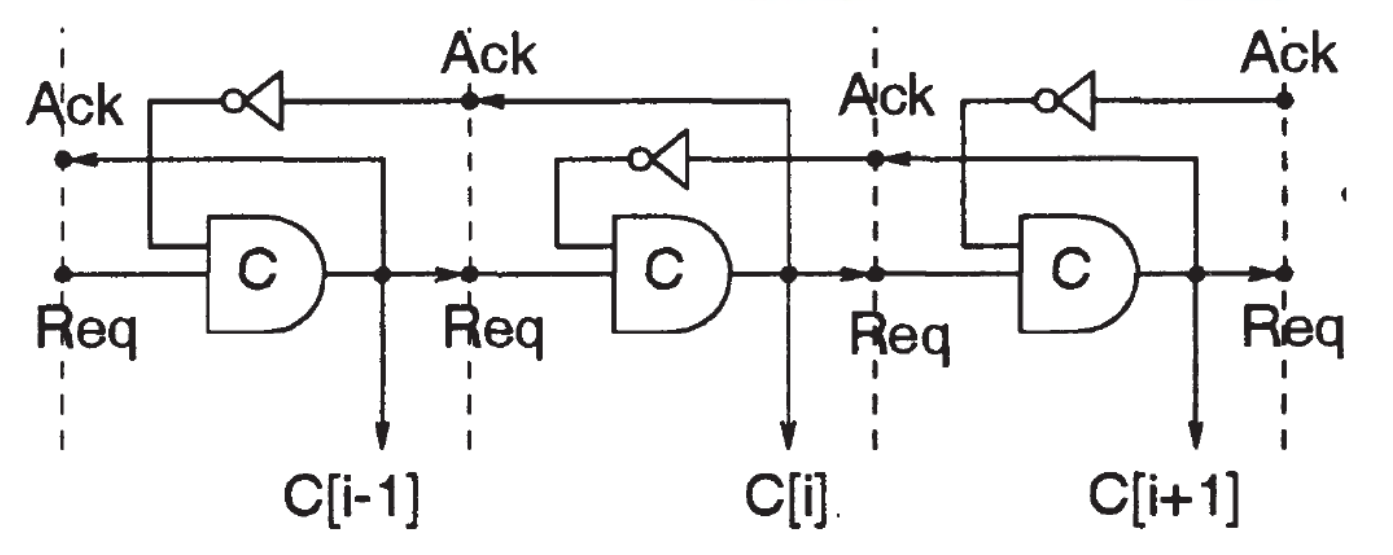
\includegraphics[width = 0.5 \textwidth]{micropipeline} \label{fig:micropipeline}
	\caption{Sutherland's basic micro-pipeline for asynchronous circuits.} 
	\label{fig:micropipeline}
\end{figure}

\section{Self-Timed Pipelines}

Self-timed pipelines ensure progress without the help of external signals
(clock). Unlike most modern processors where deep pipelines result
in large control overhead (synchronous stall signals), free elasticity in
asynchronous pipelines provide for data-driven throttling of speed and
power.

The basic micro-pipeline was developed by Ivan Sutherland (fig.
\ref{fig:micropipeline}) \cite{sutherland_cite}.
Its main pitfall is the fact that the pipeline evaluates 
\emph{at most half} of its stages at any instant.

Another family of self-timed circuits is composed of alternating computation and
interconnection blocks \cite{seger_book}. Computational blocks
use \emph{Dynamic Cascode Voltage Switch Logic} (DCVSL), a four-phase logic style,
and the interconnection blocks control handshaking.

A good reference for self-timed pipelines is \cite{micropipeline_cite}.


\begin{figure} 
	\centering
	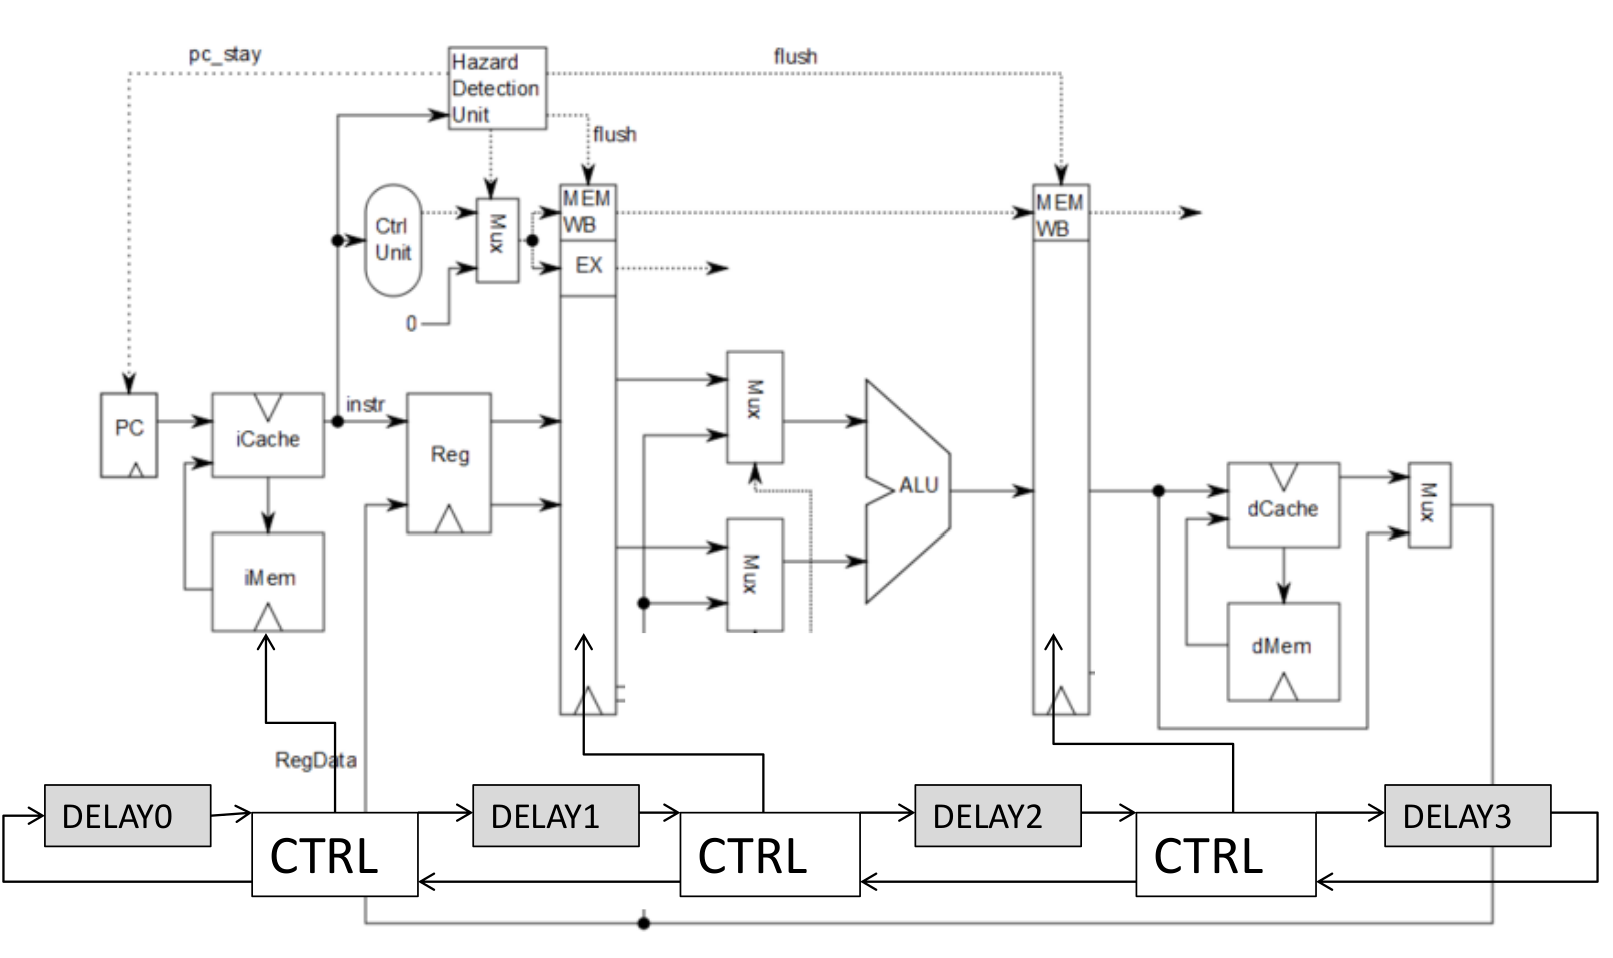
\includegraphics[width = 0.5 \textwidth]{pipeline} 
	\caption{The three-stage asynchronous pipeline implemented on Xilinx
	Virtex-5.} 
	\label{fig:pipeline}
\end{figure}

\section{The Asynchronous Pipeline Setup}

A three-stage pipeline of an in-order RISCV32UI integer processor is
implemented. A synchronous and asynchronous
version of the same pipeline was written and compared. 
The asynchronous pipeline (as in fig. \ref{fig:pipeline}) has stage registers 
implemented by flip-flops but clocked by the micro-pipeline (fig.
\ref{fig:micropipeline}). Since the stage delays may be mis-matched, \emph{no
data forwarding or speculative execution} is performed in either design.

The EECS151: FPGA Lab resource Xilinx Virtex-5 FPGA was used for the
experiments. Its basic assembly tests were used for verification and debugging, 
and the \texttt{mmult} program for benchmarking and comparing designs.

In order to implement the delay elements (DELAY0, ... DELAY3 in fig. \ref{fig:pipeline}), the
Virtex 5 primitive IODELAY was used. IODELAY can provide user-adjusted fixed
delay to Input/Output ports or to the internal fabric. The resolution of the
delay line used is about 31 ps. at 50 MHz control frequency. Fixed tap delay
requires the use control primitive IODELAYCTRL
(one each in 16 clock regions). 


\begin{figure} 
	\centering
	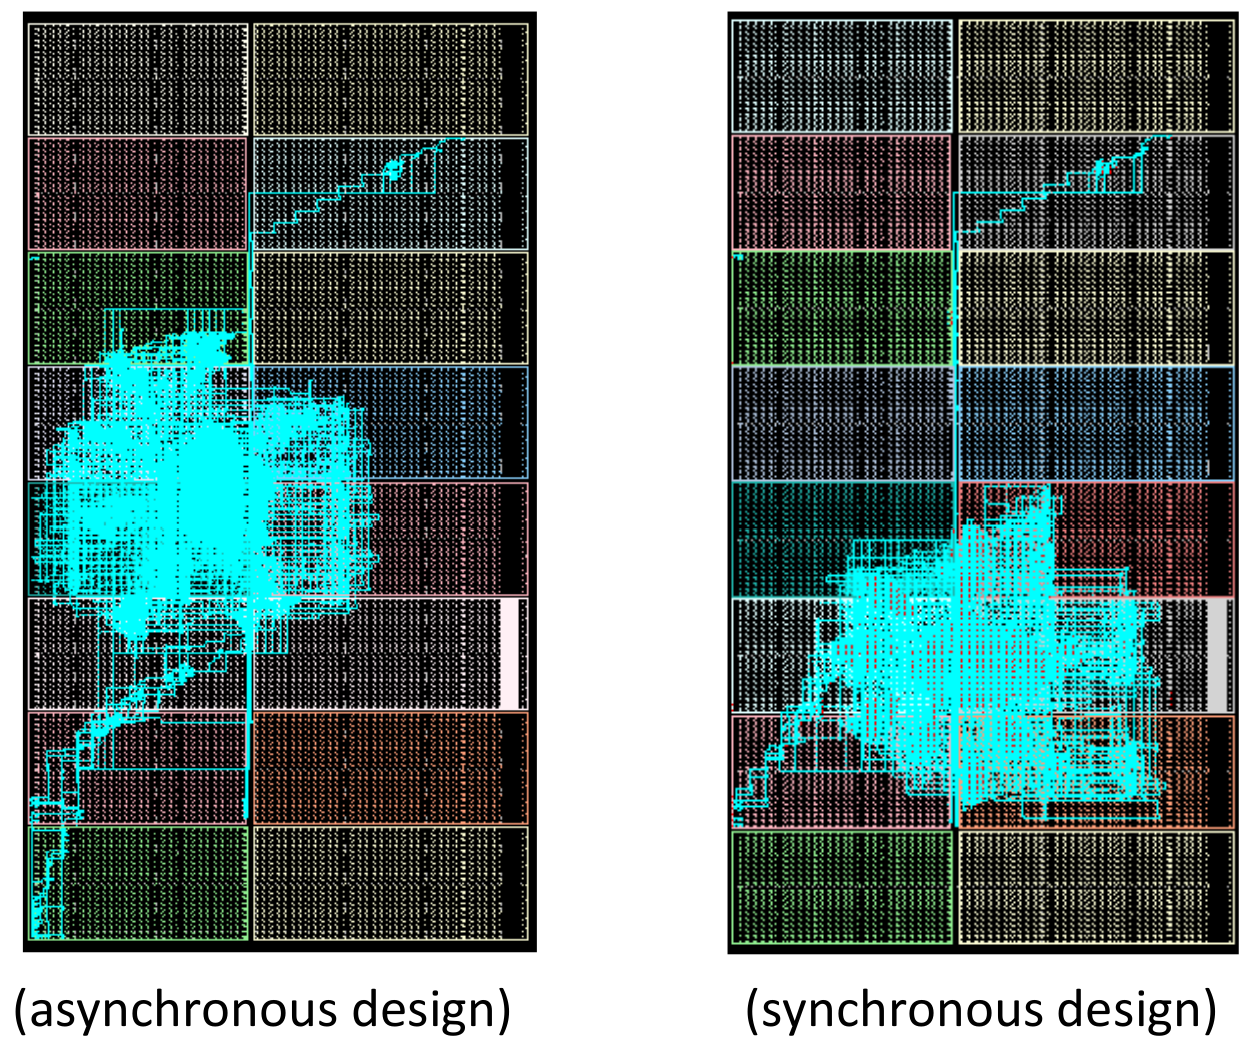
\includegraphics[width = 0.5 \textwidth]{layout}
	\caption{The routed designs: asynchronous (left) and synchronous (right).} 
	\label{fig:layout}
\end{figure}



\section{Simulation Methodology}

Preliminary Static Timing Analysis (STA) without IODELAY primitives revealed
that stage delays went up to 3.8 ns (i.e. about 3 IODELAYs). Virtex 5 requires
\emph{all clock signals to be buffered} before being clocked into a latch.
Since the buffering is performed automatically (depending on the number of
clock domain crossings), the user cannot limit the distance between 
micro-pipeline gates and IODELAYs without manually routing the entire design.

This was a significant problem: a change in the number of IODELAYs for
a stage will change the routed design unpredictably. Hence, number of IODELAYs
for \emph{each stage} must be tuned correctly at once.

With a lack of alternatives, a manual iteration schedule was followed:
\begin{enumerate}
	\item Set the number of IODELAYs for each stage.
	\item Find out the stage delays after tool-flow using STA.
	\item If the pipeline path is \emph{within limits} of the delay provided 
		by the current number of IODELAYs for all
		stages, continue. 
		If for any path the STA delay is longer than the
		maximum delay provided by IODELAYS, increment the number of IODELAYs.
		If there are many such stages, increment for the stage with least 
		number of IODELAYs. Go to Step 2.
	\item If you have Static timining delays within the limits of IODELAYs, set
		the correct tap delay for each stage.
	\item Perform assembly tests. If fail, return to Step 1 with the stage with
		smallest total IODELAY delay incremented. If the IODELAYs are already at their
		maximum delay for that stage, a new IODELAY must be added. 
	\item Benchmark \texttt{mmult} to obtain the effective throughput.
\end{enumerate}


\section{Results}
Fig. \ref{fig:layout} shows the routed wires and SLICEs for the design.
The asynchronous design has more wires towards the left edge -- to connect to
IODELAYs forced to be at the chip (IO) boundary. 

\begin{center}
\begin{tabular}{||c c c c||} 
	\hline
	\textbf{Resource} & \textbf{Sync.} & \textbf{Async.} & \textbf{Change} \\ [0.5ex] 
	\hline\hline
	SLICE Regs. & 1413 & 1446 & +33 (23 \%) \\ 
	\hline
	SLICE LUTs & 2358 & 2395 & +37 (16 \%) \\
	\hline
	BUFG/BUFGCTRL & 2 & 5 & +3 \\
	\hline
	Throughput & 67.4 MIPS & 24.1 MIPS & - 43.3 (- 64 \%) \\
	\hline
\end{tabular}
\end{center}

Clearly, the \texttt{mmult} throughput of asynchronous design was lower than 50 
\% of synchronous since only half of the micro-pipeline can be full. 
Rest of the loss can be accounted for by over-estimation of IODELAY values
(due to manual tuning) and extra latency to IODELAY at the edge of chip.
\\

Xilinx ML505/6/7 development board does not have supply resistances to measure current. Hence,
power measurements could not be performed. The difficulties in
designing the asynchronous system on a commercial synchronous machine
highlights the mismatch between conventional tools and asynchronous design.

\newpage

\appendices
% you can choose not to have a title for an appendix
% if you want by leaving the argument blank
\section{The C Gate and the Virtex-5 FPGA}
The Muller C gate is a sequential circuit element which switches only when all its inputs have
the same value.
When inputs disagree, the gate output retains its previous value.
Any multi-input C gate can be expressed as a cascade of 2-input C gates
(henceforth MULLER).
This appendix describes the MULLER gate and derives its realization on 
the Xilinx Virtex-5 FPGA.
\\

Boolean expressions of sequential elements need special notation to distinguish
between the current value and next value of signals. 
We denote both the signal and its current value by the signal name. 
Hence, $a$ denotes the value of signal 'a' at the current instant. 
Let $a'$ denote its value at the next instant and $\overline{a}$ its
logical negation. $a''$ will be the value of 'a' after $a'$.
Also, let $\oplus$, $\cdot$ and $+$ represent logical XOR, AND and OR respectively.
\\

The MULLER gate can be modelled as a latch which is transparent to one of its
inputs only when both of them agree:
\begin{equation} \label{eq:muller_c}
	\texttt{MULLER}(a,b)' = 
	\overline{(a \oplus b)} \cdot a\ +\ (a \oplus b) \cdot \texttt{MULLER}(a,b)
\end{equation}
%The C gate is the principal element of asynchronous circuits as it implements
%the indication principle -- it indicates a module to start working only when
%its inputs are ready. 
%\\

%----------------------------------------------------------------------
% Subsection: Virtex 5 primitives
\subsection{Xilinx Virtex-5 Primitives}

The Xilinx Virtex-5 FPGA contains 4 storage elements in each SLICE.
A storage element can be configured as a level-sensitive latch with input
driven by a LUT in the same SLICE. 
The latch is transparent when the control signal clock \texttt{CLK} is LOW. 
Any latch element can either be instantiated directly as a 
\textsl{Transparent Data Latch with Asynchronous Clear and Preset and Gate
Enable} (LDCPE) primitive or inferred by the Xilinx Synthesis Tool (XST).

Although XST enables optimization across modules, inferred synthesis may 
combine handshake stages to produce unwanted behaviour [TODO: experiment to
see].
For guaranteed functionality, the LDCPE primitive must be used. 
Its inputs are asynchronous clear (\texttt{CLR}) and preset
(\texttt{PRE}), gate enable (\texttt{GE}), gate (\texttt{G}) and data
(\texttt{D}):
\begin{equation}\label{eq:virtex_latch}
	\texttt{LDCPE}' = \overline{\texttt{CLR}} \cdot 
	(\texttt{PRE} + (\texttt{GE} \cdot \texttt{G}) \cdot \texttt{D}) +
	\overline{\texttt{CLR}} \cdot 
	(\overline{\texttt{GE} \cdot \texttt{G}}) \cdot \texttt{LDCPE}
\end{equation}

A straightforward way of synthesizing MULLER on Virtex-5 would be to program
a LUT for the XNOR gate $\overline{(a \oplus b)}$ and connect its output to
\texttt{CLK}.
%----------------------------------------------------------------------
% Subsection: C gate using RS and SR Latches
%----------------------------------------------------------------------

\subsection{C Gate using RS and SR Latches}

Although MULLER can be implemented by a single latch and LUT, it is prone
to spurious transitions in inputs. 
Using two latches reduces the risk of an output transition due to glitching.
A well known implementation of MULLER using RS and SR latches due to Murphy
[TODO: cite murphy] can be used for this purpose.

Both SR and RS latches have two inputs \texttt{set} (\texttt{S}) and
\texttt{reset} (\texttt{R}). 
SR latch is equivalent to the RS latch with \texttt{R} and \texttt{S} inputs
interchanged and the output inverted.
\begin{equation}\label{eq:rslatch}
	\texttt{RSLatch}(\texttt{S},\texttt{R})' 
	= \overline{\texttt{R}} \cdot (\texttt{S} + \texttt{RSLatch})
\end{equation}
\begin{equation}\label{eq:srlatch}
	\texttt{SRLatch}(\texttt{S},\texttt{R})' 
	= \texttt{S} + \overline{\texttt{R}} \cdot \texttt{SRLatch}
\end{equation}

For brevity $\texttt{MULLER}(a,b)$ is denoted by $c$. 
 One can easily simplify eqn. \ref{eq:muller_c} (using identity $x + \overline{x}
 \cdot y = x + y$ ) to obtain:
\begin{equation}\label{eq:muller_c_simplified}
\begin{split}
	\texttt{MULLER}(a,b)' &= c'\\
	&= (a \cdot b + \overline{a} \cdot \overline{b}) \cdot a 
		+ (a \cdot \overline{b} + \overline{a} \cdot b) \cdot c \\
	&= a \cdot (b + \overline{b} \cdot c) + \overline{a} \cdot b \cdot c \\
	&= a \cdot c + b \cdot (a + \overline{a} \cdot c) \\
	&= a \cdot b + (a + b) \cdot c
\end{split}
\end{equation}
To express MULLER in terms of SR and RS latches, 
observe that eqn. \ref{eq:muller_c_simplified} contains only true values of
inputs but \texttt{R} appears in both SR and RS latches (eqs. \ref{eq:srlatch}
and \ref{eq:rslatch}) as $\overline{R}$. 
Hence, \texttt{R} of the latches will be $\overline{a}$ or $\overline{b}$.
Only the expression for RS latch (eqn. \ref{eq:rslatch}) has a minterm containing both \texttt{R}
and \texttt{S}, which will produce the minterm $ a \cdot b $ in eqn. \ref{eq:muller_c_simplified}.
\\
Therefore, the RS latch appears in the first stage producing the minterms $a
\cdot b$ and $a \cdot c$ or $b \cdot c$ (depending on \texttt{R} being
$\overline{a}$ or $\overline{b}$ respectively). 
The SR latch forms the second stage.
Since \texttt{S} appears alone in its expression, we connect the RS output
to \texttt{S} and the input other than \texttt{R} of previous stage to the
\texttt{R} of the second stage.

Representing the RS output by $p$ and the subsequent SR output by $q$,
we have:
\begin{equation}\label{eq:muller_rs}
\begin{split}
	\texttt{RSLatch}(\texttt{S}=a, \texttt{R}=\overline{b}) &= p' = a \cdot b + b \cdot p \\
	\texttt{SRLatch}(\texttt{S}=p, \texttt{R}=\overline{a}) &= q' = p + a \cdot q \\
\end{split}
\end{equation}
From above, we have $q'' = p' + a' \cdot q' = (a \cdot b + b \cdot p) + 
a' \cdot (p + a \cdot q)$. 
Assuming input steady state i.e.\ $a'' = a' = a$ and $b'' = b' = b$,
\begin{equation}
\begin{split}
	q''& = a \cdot b + a \cdot p + b \cdot p + a \cdot q\\
	&= a \cdot b \cdot (1 + q) + (a + b ) \cdot p + a \cdot q\\
	&= a \cdot b + (a + b ) \cdot p + a \cdot q + a \cdot b \cdot q\\
	&= a \cdot b + (a + b ) \cdot p + (a + b) \cdot a \cdot q\\
	&= a \cdot b + (a + b ) \cdot (p + a \cdot q)\\
	&= a \cdot b + (a + b ) \cdot q'
\end{split}
\end{equation}

This proves the equivalence of the latch pair (eqn. \ref{eq:muller_rs}) to MULLER
(eqn. \ref{eq:muller_c_simplified}).

It may appear that the heuristic used to connect the pair just happened to
prove equivalent to MULLER. 
However, the circuit really was synthesized using reductions on a 
Signal Transition Graphs (STG) specification [TODO: cite murphy]. 
STGs are directed graphs with nodes corresponding to minterms in eqn.
\ref{eq:muller_c_simplified} [TODO: Find citation]. 
The synthesis algorithm does something similar to matching leaf nodes of the
latch STGs with that of MULLER -- like our heuristic [TODO: Find
citation]. 
Also, note that the difference of SR and RS latch expressions (eqs.
\ref{eq:srlatch} and \ref{eq:rslatch}) helped using the heuristic. 
Though an RS latch can be converted to SR latch easily, it would be much harder
to build the pair using 2 SR latches.

The LDCPE primitive can be easily configured as RS and SR latches. 
To set $\texttt{LDCPE} = \texttt{RSLatch}(\texttt{S}, \texttt{R})$ by comparing
eqs. \ref{eq:virtex_latch} and \ref{eq:rslatch}, we set
$\texttt{CLR} = \texttt{R}$ and $\overline{\texttt{GE} \cdot \texttt{G}} = 1$.
Then, $\texttt{PRE} = \texttt{S}$.
Similarly, for $\texttt{SRLatch}$ set $\overline{\texttt{CLR}} = 1,
 (\texttt{GE} \cdot \texttt{G}) = \texttt{R}, \texttt{D} = 0$ and $\texttt{PRE}
 = \texttt{S}$.


\section{Energy and Entropy of Asynchronous Circuits} \label{appendix_entropy}
This appendix sketches a proof of a lower bound on the scalability of
energy dissipated by an asynchrnonous circuit in terms of the entropy of its specification.

%----------------------------------------------------------------------
% Subsection: Specification and Entropy
%----------------------------------------------------------------------
\subsection{Circuit Specification and Entropy}

Analogous to a structural or behavioral description of a synchronous system,
asynchronous circuits are specified using a process algebra formalism.
Any circuit description requires an \emph{alphabet} of signals 
$\mathbb{C} = \{\mathbb{I}, \mathbb{S}, \mathbb{O}\}$ composed of  
inputs ($\mathbb{I}$), outputs ($\mathbb{O}$) and internal \emph{state}
signals ($\mathbb{S}$). 

An asynchronous circuit is described as a collection of communicating \emph{processes} --
sequential programs executing simultaneously on separate machines and 
synchronizing by passing messages. 

A \emph{statement}, denoted by block letters except $G$, is a boolean assignment
where a state/output signal is assigned the value of a boolean expression 
of any number of signals. $A; B$ is a sequential process 
where statement $B$ begins only after $A$ completes. 
A \emph{guard} ($G, G_1, G_2, ...$) is a boolean condition composed of any number of
signals, used to implement control flow. There are two control structures:
\begin{itemize}
	\item \textbf{Deterministic Selection} Denoted by 
		$[ G_1 \to S_1\ \Box\ G_2 \to S_2\ \Box\ ... \Box\ G_n \to S_n ]$  
		where at most one guard $G_1 ... G_n$ is true at any instant. 
		The program waits until a guard becomes true. 
		If $G_i$ is true, only $S_i$ executes.

	\item \textbf{Non-Deterministic Selection} Denoted by 
		$[ G_1 \to S_1\ |\ G_2 \to S_2\ |\ ... |\ G_n \to S_n ]$.
		Same as Deterministic Selection, except when more than one
		guards are true, any one of them is selected. The selection criteria
		is not necessarily random and can be assumed to be demonic for the
		circuit correctness.
\end{itemize}
A \emph{repetition} on a control structure is denoted by '$*[...]$': 
the control structure is repeatedly executed until no guards are true.
$S_1 || S_2$ denotes \emph{concurrent} execution, where the statements are executed
in any order and ensures \emph{weak fairness} (i.e. any action that is enabled
to execute and stays enabled will eventually execute).

Any of the guarded statements $S_1... S_n$ in the examples above could be 
control structures, their repetitions, sequential processes or concurrent processes themselves. 
Finally, for message passing, a special data structure \emph{channel} (denoted
by $\mathbf{1}, \mathbf{2}...$) is used. 
At any instant, at most one statement shall read from or write to a channel.
A read statement $\mathbf{1} ? v$ reads the value from the channel and stores
it in signal $v$. A write statement $\mathbf{1} ! G$ evaluates the boolean
expression $G$ and write the value to channel $\mathbf{1}$. A read and write
statement waits till channel is full or empty respectively.
\\

We postulate that any asynchronous circuit can be completely described 
by a process P of the form:
\begin{equation} \label{eq:basic_csp}
	P = *[[ G_1 \to A_1; X_1 \Box\ G_2 \to A_2; X_2 \Box\ ... \Box\ G_n \to
	A_n; X_n ]]
\end{equation}
where $A_1.. A_n$ are either \textbf{skip} or message passing
statements, $X_1... X_n$ are simple assignments where the value assigned is a
boolean constant \cite{entropy_paper}.
This essentially means all computation by the circuit is captured by
evaluation of guard conditions alone.
\\

Let $Z_i$ be a random variable for the i\textsuperscript{th} statement executed by P. 
The probability distribution for $Z_i$ can be numerically calculated assuming a
prior input distribution or estimated by profiling actual traces of execution.
\\

\begin{defn}[Entropy]
	Let $Z = (Z_1, Z_2, ... Z_m)$ be a sequence of $m$ discrete random variables over
	range $S_m$ with joint probability mass function $\Pr(Z_1, Z_2, ... Z_m)$. 
	The entropy of the sequence is 
	\begin{equation}
		H(Z_1, Z_2, ... Z_m) = - \sum_{\mathclap{(z_{1...m}) \in S_m}} 
				\Pr(z_1 ... z_m) \log_2{\Pr(z_1... z_m)}
	\end{equation}
\end{defn}
\begin{defn}[Entropy of a Process]
	The entropy of a process P which executes sequence of statements $Z_1, Z_2, ...$ is 
	\begin{equation}
		H(P) = \lim_{m \to \infty}{ \sup \frac{1}{m} H(Z_1, Z_2, ... Z_m)}
	\end{equation}
\end{defn}

P has about $n$ statements $X_{1...n}$ ($A_{1...n}$
are mostly \textbf{skips} as circuits often have a lot of signal-level
parallelism), hence $Z_1, Z_2, ...$ can have values n distinct values. 
Therefore, their entropies are bounded $H(Z_1), ... H(Z_2) \le \log_2{n}$.
Hence, the entropy of the process P exists as its a limit of the supremum
of a bounded sequence:
\begin{equation}
	\frac{1}{m} H(Z_1...Z_m) \le \frac{1}{m} (H(Z_1) + ... + H(Z_m)) \le
	\log_2{n}
\end{equation}

%----------------------------------------------------------------------
% Subsection: Energy and Entropy
%----------------------------------------------------------------------
\subsection{Energy Index of Asynchronous Circuits}

A CMOS circuit has three main sources of energy dissipation: leakage currents,
short circuit currents and dynamic switching currents flowing between the rails.
An \emph{operation} is defined as a \emph{finite} sequence of input transitions
within a finite time. The input values may not be provided, only the number of
transitions and their times must be specified \cite{trace_theory}.
Assuming most of the circuit is implemented using static CMOS (dynamic nodes
are usually pulled to rail by weak feedback to prevent soft errors) and 
designed to have low leakage, we can estimate the total energy expended
\textbf{in one operation} of the circuit:
\begin{equation}
	E_T \approx E_{sw} = \sum_{i} n_i C_i V_{DD}^2 
\end{equation}

Here, all nodes (indexed by $i$) have capacitance $C_i$ and switch
 LOW to HIGH $n_i$ times during one operation.
The intermediate nodes of stacked transistors are ignored (they are usually smaller than drain
capacitances and charge to values lower than $V_{DD}$).

It is worthwhile to note differences of this energy model to that of a
synchronous circuit. The switching factor $n_i$ is an integer rather than a probability. 
Also, a well-defined operation requires that outputs stabilize within
finite time after the inputs switch. A special class of asynchronous circuits 
are required to avoid metastability \cite{seger_book}.
\\

The \emph{energy index} of the circuit is defined as $K = \sum_i n_i C_i$.
Energy indices are additive: the index of a circuit is a sum of energy indices
of all its sub-circuits. The energy index of a CSP $P$ is denoted by $C(P)$.

A central assertion of this model is that parallel sub-circuits with no
synchronization require no extra energy. 
This is reasonable since no synchronization essentially means no
extra circuitry, only extra wires for common signals. 

Since asynchronous circuits compute only when required, the chances of a sub-circuit 
turning on and consuming switching energy depends on the inputs. If probability
of sub-circuits $P_1$ and $P_2$ turning on during one operation are $w_1$
and $w_2$, then the total energy index is $K = w_1 K_1 + w_2 K_2$.

The three possible ways of enforcing order in CSP are: sequential ordering
(;), choice (deterministic and non-deterministic) and message-passing. Energy 
models of implementing each of these are supplied without proof, please refer 
\cite{entropy_paper} for the same.

Receiving and transmitting $N$-bit values over a channel requires energy
index proportional to $N$. 
A guarded choice $P = *[[G_1 \to P_1 \Box\ ...\ \Box\ G_n \to P_n]]$
entails an extra energy index $\propto \log_2 {n}$ over executing the guarded 
statements concurrently 
$Q = *[[G_1 \to A_1 ]]\ ||\ *[[G_2 \to A_2]]\ ...\ ||\ *[[ G_n \to A_n]]$.
This is because we can implement the guarded choice using concurrent
statements and extra $\log_2{n}$ single-bit channels for message-passing
\cite{entropy_thesis}.
\\

Now consider the program P from from eqn. \ref{eq:basic_csp} with $n = 2$. The energy index
can be evaluated as 
\begin{equation}
\begin{split}
	C(P) = C(G_1) + C(G_2) + k \log_2{2} +\\
	w_1 C(A_1; X_1) + w_2 C(A_2; X_2).
\end{split}
\end{equation}
Here $k$ is a technology constant. Notice that the energy indices of all the
guards are added irrespective of their probabilities being true.

Without loss of generality, assume $w_1 \ge w_2$. 
Now consider the following modification to the program:
\begin{equation}
	Q = *[[ G_1 \to A_1; X_1 \Box\ [ \overline{G_1} G_2 \to A_2; X_2] ]]
\end{equation}

The modified energy index is 
\begin{equation}
\begin{split}
	C(Q) &= C(G_1) + w_1 C(A_1; X_1) + k \log_2{2} +\\
		& (1 - w_1) (C(G_2) + u + w_2 C(A_2; X_2)) \\
		&\approx C(G_1) + (1 - w_1) C(G_2) + k \log_2{2} + \\
		& w_1 C(A_1; X_1) + (1 - w_1) w_2 C(A_2; X_2)\\
		&< C(P)
\end{split}
\end{equation}

Here the constant $u$ is the fixed energy index to compute a logical
negation and a logical AND of the result (usually negligible). 
Therefore, re-structuring the program P such that a more common
guard executes before a less common guard saves overall energy.

For the general case ($n$ guarded statements), assume 
P is re-structured to a tree of cascaded guarded statements Q as above. 
Let $Y_i = A_i; X_i$ denote the guarded statements of P.
Then, for a particular $Y_i$ of P there is a corresponding order of guard
evaluation through the tree in Q which ends in the leaf node for $Y_i$.
At a depth $d$ in the tree of Q, energy will be dissipated by \emph{all guard
evaluations} at that depth. Let $S(Y_i) \subset \{G_1, G_2, ... G_n\}$ be the set
of all guards that were evaluated by Q to reach leaf node for $Y_i$. Further,
let $d(Y_i)$ denote the depth of the leaf node $Y_i$ in the tree of Q, and let
$n_1(Y_i), n_2(Y_i), ... n_{d(Y_i)}(Y_i)$ be the number of guards that were
evaluated at depth 1, 2, ... $d(Y_i)$ respectively.

Then, the energy index for evaluating $Y_i$ is given by
\begin{equation}
	C_{Y_i}(Q) = \sum_{G \in S(Y_i)} C(G) + \sum_{j = 1}^{d(Y_i)} k 
	\log_2{n_j(Y_i)} + C(Y_i)
\end{equation}
and the energy index for evaluating $Y_{1...m} = Y_1, Y_2, ... Y_m$ by Q is
$C_{Y_{1...m}}(Q) = \sum_{i = 1}^{m} C_{Y_i}(Q)$. 

\begin{defn}[Energy Index per Operation]
	$\Pr(y_1,...y_m)$ is the probability of the sequence of statements $(y_1, y_2, ...y_m)$ 
	being executed by P. 
	Then, the energy index \textbf{per operation} of Q is defined as the expected average
	energy index of a chain of operations 
	\begin{equation}
		C(Q) = \lim_{m \to \infty} \frac{1}{m} \sum_{(y_1,...y_m)} \Pr(y_1,...y_m) C_{Y_{1...m}}(Q)
	\end{equation}
\end{defn}

The above expression is really the average energy index in the limit of long
chains. Assuming the statements $y_1, y_2, ...$ are independent and identically
distrubuted, using the law of large numbers we have:
\begin{equation}\label{eqn:simplified_cost}
	C(Q) = \mathbb{E} \Big[\sum_{G \in S(Y)} C(G) + C(Y) \Big] 
		+ k\ \mathbb{E} \Big[\sum_{j=1}^{d(Y)} \log_2{n_{j}(Y)} \Big] 
\end{equation}

Here, $\mathbb{E[\cdot]}$ denotes the expectation with respect to the sequence
of statements $(y_1,...y_m)$ having joint probability distribution of
$\Pr(y_1,...y_m)$.

Now, the path to $Y$ is determined by which of the guards resolved true at each
depth. Since there are $n_i(Y)$ distinct guards at depth $i$, we can identify
the true guard at depth $i$ by a binary number $\log_2{n_i(Y)}$ bits wide. The
entire path is then a list of such numbers in total 
$\sum_{i=1}^{d(Y)} \log_2 n_i(Y)$ bits wide (call it $I(Y)$).
Since all statements are leaf nodes, the binary nnumber $I(Y)$ cannot be a
prefix to any $I(J), J \ne Y$. Hence, $I(Y)$ is a prefix code for $Y$, and 
$\mathbb{E}[\sum_{i=1}^{d(Y)} \log_2n_i(Y)]$ is the average code-length. 
A fundamental result from by C. Shannon from Information Theory states that the
average code length of any prefix code is atleast the entropy of the alphabet
\cite{shannon_paper}. 
Hence $\mathbb{E}[\sum_{i=1}^{d(Y)} \log_2n_i(Y)] \ge H(Y)$. 

Therefore, we have 
\begin{equation}
	C(Q) \ge (\sum_{i=1}^{n} w_i C(Y_i) + \mathbb{E}[\sum_{G \in S(Y)} C(G)] ) + k H(Y)
\end{equation}
\\

The first term in parenthesis is the \emph{indispensable} cost for evaluating the guards
and executing the statements. As such, asynchronous paradigm does not provide
any major benefits.

The last term relates to the \emph{scalability}
of energy with the design size. Unlike synchronous systems where the energy scalability
factor is linear (or polynomial) in size, an optimally designed
asynchronous circuit scales linearly with the \emph{entropy} of the system. 
This shows the \emph{asymptotic} utility of asynchronous circuits
for energy efficiency in large systems.
\\

In this sketch, several details about methods of specification and
transformation were not provided. This theory is very thoroughly 
developed in \cite{entropy_thesis} \cite{entropy_paper}. 


% Can use something like this to put references on a page
% by themselves when using endfloat and the captionsoff option.
\ifCLASSOPTIONcaptionsoff
  \newpage
\fi

\begin{thebibliography}{1}



\bibitem{seger_book}
	J.~A. Brzozowski and C-J.~H. Seger, \emph{Asynchrnonous Circuits},
		Monographs in Computer Science, Springer 1995.

\bibitem{async_test_survey}
	H.~Hulgaard, S.~M. Burns, G.~Borriello, \emph{Testing asynchronous
		circuits: A survey}, Integration, the VLSI Journal, Volume 19, Issue 3,
		1995, Pages 111-131.

\bibitem{async_c_test}
	J.~A. Brzozowski and K.~ Raahemifar, \emph{Testing C-elements is not
		elementary}, Proceedings Second Working Conference on Asynchronous
		Design Methodologies, London, 1995, pp. 150-159.

\bibitem{japan_fpga_paper}
	J.~Furushima, M.~Nakajima, H.~ Saito, \emph{Design of an Asynchronous
		Processor with bundled-data implementation on an commercial FPGA},
		Informaticam Vol. 90, No. 4, 2016.

\bibitem{japan_1}
	M.~Tranchero and L.~M. Reyneri, \emph{Exploiting synchronous 
		placement for asynchronous circuits onto commercial FPGAs}
		, Proc. FPL, pp.622–625, 2009.
		
\bibitem{japan_2}
		Q.~T. Ho et al.,\emph{Implementing Asynchronous Circuits
		on LUT Based FPGAs}, Proc. FPL, pp.36–46, 2002.

\bibitem{japan_3}
		H.~Saito et al., \emph{A Floorplan Method for Asynchronous Circuits
		with Bundled-data Implementation on FPGAs}, Proc. ISCAS, pp.925–928, 2010.

\bibitem{japan_4}
	K.~Takizawa et al., \emph{A Design Support Tool Set for
		Asynchronous Circuits with Bundled-data Implemen-
		tation on FPGAs}, Proc. FPL, pp.1–4, September
		2014.

\bibitem{japan_5}
	N.~Minas et al., \emph{FPGA Implementation of an
		Asynchronous Processor with Both Online and Of-
		fline Testing Capabilities}, Proc. Async, pp.128–137,
		2008.

\bibitem{sutherland_cite}
		I.~E. Sutherland, \emph{Micropipelines} Commun. ACM 32, 6 (June 1989),
		720-738.

\bibitem{micropipeline_cite}
		T.~E. Williams, \emph{Analyzing and improving the latency and throughput
		performance of self-timed pipelines and rings,} [Proceedings] 1992 IEEE
		International Symposium on Circuits and Systems, San Diego, CA, 1992,
		pp. 665-668 vol.2.

\bibitem{trace_theory}
	R.~Manohar, \emph{The entropy of traces in parallel computation} in IEEE
		Transactions on Information Theory, vol. 45, no. 5, pp. 1606-1608, Jul
		1999.

\bibitem{shannon_paper}
	C. Shannon, \emph{ A mathematical theory of communication},
	In Bell Systems Tech. J., volume 27, pages 379-423,1948.

\bibitem{entropy_paper}
	J.~A. Tierno, R.~Manohar, and A.~J. Martin. \emph{The Energy and
	Entropy of VLSI Computations} In Proceedings of the 2nd International
	Symposium on Advanced Research in Asynchronous Circuits and Systems (ASYNC
	'96). IEEE Computer Society, Washington, DC, USA, 1996.

\bibitem{entropy_thesis}
	J.~A. Tierno, \emph{An energy-complexity model for VLSI
	computations} Dissertation (Ph.D.), California Institute of Technology.
	1995.

\end{thebibliography}





% trigger a \newpage just before the given reference
% number - used to balance the columns on the last page
% adjust value as needed - may need to be readjusted if
% the document is modified later
%\IEEEtriggeratref{8}
% The "triggered" command can be changed if desired:
%\IEEEtriggercmd{\enlargethispage{-5in}}
% references section

% that's all folks
\end{document}


